% Options for packages loaded elsewhere
\PassOptionsToPackage{unicode}{hyperref}
\PassOptionsToPackage{hyphens}{url}
%
\documentclass[
  11pt,
]{article}
\usepackage{amsmath,amssymb}
\usepackage{iftex}
\ifPDFTeX
  \usepackage[T1]{fontenc}
  \usepackage[utf8]{inputenc}
  \usepackage{textcomp} % provide euro and other symbols
\else % if luatex or xetex
  \usepackage{unicode-math} % this also loads fontspec
  \defaultfontfeatures{Scale=MatchLowercase}
  \defaultfontfeatures[\rmfamily]{Ligatures=TeX,Scale=1}
\fi
\usepackage{lmodern}
\ifPDFTeX\else
  % xetex/luatex font selection
    \setmainfont[]{Times New Roman}
\fi
% Use upquote if available, for straight quotes in verbatim environments
\IfFileExists{upquote.sty}{\usepackage{upquote}}{}
\IfFileExists{microtype.sty}{% use microtype if available
  \usepackage[]{microtype}
  \UseMicrotypeSet[protrusion]{basicmath} % disable protrusion for tt fonts
}{}
\makeatletter
\@ifundefined{KOMAClassName}{% if non-KOMA class
  \IfFileExists{parskip.sty}{%
    \usepackage{parskip}
  }{% else
    \setlength{\parindent}{0pt}
    \setlength{\parskip}{6pt plus 2pt minus 1pt}}
}{% if KOMA class
  \KOMAoptions{parskip=half}}
\makeatother
\usepackage{xcolor}
\usepackage[margin=1in]{geometry}
\usepackage{color}
\usepackage{fancyvrb}
\newcommand{\VerbBar}{|}
\newcommand{\VERB}{\Verb[commandchars=\\\{\}]}
\DefineVerbatimEnvironment{Highlighting}{Verbatim}{commandchars=\\\{\}}
% Add ',fontsize=\small' for more characters per line
\usepackage{framed}
\definecolor{shadecolor}{RGB}{248,248,248}
\newenvironment{Shaded}{\begin{snugshade}}{\end{snugshade}}
\newcommand{\AlertTok}[1]{\textcolor[rgb]{0.94,0.16,0.16}{#1}}
\newcommand{\AnnotationTok}[1]{\textcolor[rgb]{0.56,0.35,0.01}{\textbf{\textit{#1}}}}
\newcommand{\AttributeTok}[1]{\textcolor[rgb]{0.13,0.29,0.53}{#1}}
\newcommand{\BaseNTok}[1]{\textcolor[rgb]{0.00,0.00,0.81}{#1}}
\newcommand{\BuiltInTok}[1]{#1}
\newcommand{\CharTok}[1]{\textcolor[rgb]{0.31,0.60,0.02}{#1}}
\newcommand{\CommentTok}[1]{\textcolor[rgb]{0.56,0.35,0.01}{\textit{#1}}}
\newcommand{\CommentVarTok}[1]{\textcolor[rgb]{0.56,0.35,0.01}{\textbf{\textit{#1}}}}
\newcommand{\ConstantTok}[1]{\textcolor[rgb]{0.56,0.35,0.01}{#1}}
\newcommand{\ControlFlowTok}[1]{\textcolor[rgb]{0.13,0.29,0.53}{\textbf{#1}}}
\newcommand{\DataTypeTok}[1]{\textcolor[rgb]{0.13,0.29,0.53}{#1}}
\newcommand{\DecValTok}[1]{\textcolor[rgb]{0.00,0.00,0.81}{#1}}
\newcommand{\DocumentationTok}[1]{\textcolor[rgb]{0.56,0.35,0.01}{\textbf{\textit{#1}}}}
\newcommand{\ErrorTok}[1]{\textcolor[rgb]{0.64,0.00,0.00}{\textbf{#1}}}
\newcommand{\ExtensionTok}[1]{#1}
\newcommand{\FloatTok}[1]{\textcolor[rgb]{0.00,0.00,0.81}{#1}}
\newcommand{\FunctionTok}[1]{\textcolor[rgb]{0.13,0.29,0.53}{\textbf{#1}}}
\newcommand{\ImportTok}[1]{#1}
\newcommand{\InformationTok}[1]{\textcolor[rgb]{0.56,0.35,0.01}{\textbf{\textit{#1}}}}
\newcommand{\KeywordTok}[1]{\textcolor[rgb]{0.13,0.29,0.53}{\textbf{#1}}}
\newcommand{\NormalTok}[1]{#1}
\newcommand{\OperatorTok}[1]{\textcolor[rgb]{0.81,0.36,0.00}{\textbf{#1}}}
\newcommand{\OtherTok}[1]{\textcolor[rgb]{0.56,0.35,0.01}{#1}}
\newcommand{\PreprocessorTok}[1]{\textcolor[rgb]{0.56,0.35,0.01}{\textit{#1}}}
\newcommand{\RegionMarkerTok}[1]{#1}
\newcommand{\SpecialCharTok}[1]{\textcolor[rgb]{0.81,0.36,0.00}{\textbf{#1}}}
\newcommand{\SpecialStringTok}[1]{\textcolor[rgb]{0.31,0.60,0.02}{#1}}
\newcommand{\StringTok}[1]{\textcolor[rgb]{0.31,0.60,0.02}{#1}}
\newcommand{\VariableTok}[1]{\textcolor[rgb]{0.00,0.00,0.00}{#1}}
\newcommand{\VerbatimStringTok}[1]{\textcolor[rgb]{0.31,0.60,0.02}{#1}}
\newcommand{\WarningTok}[1]{\textcolor[rgb]{0.56,0.35,0.01}{\textbf{\textit{#1}}}}
\usepackage{longtable,booktabs,array}
\usepackage{calc} % for calculating minipage widths
% Correct order of tables after \paragraph or \subparagraph
\usepackage{etoolbox}
\makeatletter
\patchcmd\longtable{\par}{\if@noskipsec\mbox{}\fi\par}{}{}
\makeatother
% Allow footnotes in longtable head/foot
\IfFileExists{footnotehyper.sty}{\usepackage{footnotehyper}}{\usepackage{footnote}}
\makesavenoteenv{longtable}
\usepackage{graphicx}
\makeatletter
\def\maxwidth{\ifdim\Gin@nat@width>\linewidth\linewidth\else\Gin@nat@width\fi}
\def\maxheight{\ifdim\Gin@nat@height>\textheight\textheight\else\Gin@nat@height\fi}
\makeatother
% Scale images if necessary, so that they will not overflow the page
% margins by default, and it is still possible to overwrite the defaults
% using explicit options in \includegraphics[width, height, ...]{}
\setkeys{Gin}{width=\maxwidth,height=\maxheight,keepaspectratio}
% Set default figure placement to htbp
\makeatletter
\def\fps@figure{htbp}
\makeatother
\setlength{\emergencystretch}{3em} % prevent overfull lines
\providecommand{\tightlist}{%
  \setlength{\itemsep}{0pt}\setlength{\parskip}{0pt}}
\setcounter{secnumdepth}{5}
\ifLuaTeX
  \usepackage{selnolig}  % disable illegal ligatures
\fi
\usepackage{bookmark}
\IfFileExists{xurl.sty}{\usepackage{xurl}}{} % add URL line breaks if available
\urlstyle{same}
\hypersetup{
  pdftitle={NBA Hall of Fame Prediction},
  pdfauthor={Justin Mai},
  hidelinks,
  pdfcreator={LaTeX via pandoc}}

\title{NBA Hall of Fame Prediction}
\author{Justin Mai}
\date{2025-05-20}

\begin{document}
\maketitle

{
\setcounter{tocdepth}{2}
\tableofcontents
}
\newpage

\section{Abstract}\label{abstract}

\newpage

\section{Introduction}\label{introduction}

The NBA Hall of Fame inducts the most influential players, coaches,
teams, and referees yearly. There have only been just over 150 NBA
players inducted to the Hall of Fame which started with the inaugural
class of 1959. So what classifies an NBA player as a Hall of Famer
compared to other NBA players? This research paper will identify the
probability of current NBA players one day making the Hall of Fame based
on historical trends.

\subsection{Accolades and Awards}\label{accolades-and-awards}

A common debate within the basketball community is the infamous ``LeBron
vs.~Michael Jordan'' debate to crown on player as the Greatest of All
Time (G.O.A.T.). Analysts will often start with the quantitative in game
statistics by looking at all time averages for both players. Looking at
the primary statistics, throughout Jordan's career, he averaged \(30.1\)
points per game, \(6.2\) rebounds per game, and \(5.3\) assists per
game. On the other end, LeBron averages \(27.0\) points per game,
\(7.5\) rebounds per game, and \(7.4\) assists per game. While Jordan
has the edge on scoring, LeBron has the edge in the other primary
statistics so its difficult to make a clear conclusion based on this.
However, this isn't the primary argument for both players, if you've
ever been part of this debate you'll often hear the notion that ``Jordan
went 6 for 6 in championship games''. The accolades and awards that each
player compiles is often the primary argument.

While there is no clear calculator for identifying if a player will make
the Hall of Fame, in all cases, accolades and awards will be a
significant predictor to identifying HOFers. These accolades will
consist of \textbf{Regular Season MVPs, Championship Wins, Finals MVPs,
All-NBA Selections, All-Star Selections, End-of-Season Awards} and
possibly much more. These awards all signify the impact that a player
has had on their respective teams, demonstrating how their contribution
leads to the team's success.

\subsection{Player Impact / Other
Considerations}\label{player-impact-other-considerations}

Within the G.O.A.T debate, a primary argument for LeBron would be his
longevity and consistent impact on the game and the teams he goes to,
the qualitative factors that goes beyond the box score and award counts.
While accolades and awards provide a quantitative summary of a player's
career, qualitative aspects such as leadership, clutch performances,
career longevity, influence on team culture, and global popularity often
shape the broader legacy of a player.

For example, LeBron's ability to lead multiple franchises to the NBA
Finals---winning championships with three different teams is a testament
to his versatility and value as a player. Similarly, players like Allen
Iverson and Vince Carter are celebrated not only for their statistics
and accolades, but also for their cultural impact, influence on future
generations, and overall contribution to the evolution of the game.

When making predictions for Hall of Fame inductees, there are also many
traits outside of the box score that contributes to the selection
process. However, this type of impact often correlates with the
accolades and overall quantitative statistics so it will be contributing
factor within the analysis. Something like longevity will also be taken
into account through the number of years they played all together and
the number of years they played for one team.

\section{Methods}\label{methods}

\subsection{Data Collection}\label{data-collection}

The data collected starts with all \textbf{5311} players who have played
at least one game in the NBA since 1947 (when it was known as the BAA)
to 2025. The data was collected by a Kaggle user named \emph{Sumitro
Datta} in the page
\textbf{\href{https://www.kaggle.com/datasets/sumitrodatta/nba-aba-baa-stats?select=Player+Career+Info.csv}{NBA
Stats (1947-present)}}. The data was gathered using IMPORTHTML from
Google Sheets on Basketball-Reference's Play Index now known as
\textbf{\href{https://stathead.com/}{Stathead}}.

\subsection{Data Manipulation}\label{data-manipulation}

The majority of our data manipulation process in creating the primary
dataset we would use was done using Python and JupyterNotebook.

With the several datasets provided, there were different statistics that
we required merging before curating our logistic regression model. We
first looked at \textbf{player accolades} to get player award counts
from the All-star, Awards, and End-Season-Teams tables. We turned each
award into its own column so that every observation would be the number
of that specific award a player won. We then combined these awards with
the number of all-star games and number of seasons a player played in
the NBA. This was all joined using a player's \emph{player\_id}

We then wanted to combine in-game player statistics with the accolades
dataset. These statistics will consist of both total career statistics
and player averages to give us flexibility in choosing our model. For
many of the players, there were NA values for some statistics that
weren't yet accounted for (such as 3 pointers and some awards). These NA
values were replaced with 0.

\subsection{Data Transformation}\label{data-transformation}

\begin{Shaded}
\begin{Highlighting}[]
\NormalTok{df }\OtherTok{\textless{}{-}} \FunctionTok{read.csv}\NormalTok{(}\StringTok{"data/final.csv"}\NormalTok{)}
\end{Highlighting}
\end{Shaded}

\begin{Shaded}
\begin{Highlighting}[]
\NormalTok{train }\OtherTok{\textless{}{-}} \FunctionTok{read.csv}\NormalTok{(}\StringTok{"data/train.csv"}\NormalTok{)}

\NormalTok{train}\SpecialCharTok{$}\NormalTok{mvp\_flag }\OtherTok{=} \FunctionTok{factor}\NormalTok{(}\FunctionTok{ifelse}\NormalTok{(train}\SpecialCharTok{$}\NormalTok{nba.mvp }\SpecialCharTok{\textgreater{}} \DecValTok{0}\NormalTok{, }\DecValTok{1}\NormalTok{, }\DecValTok{0}\NormalTok{))}

\NormalTok{test }\OtherTok{\textless{}{-}} \FunctionTok{read.csv}\NormalTok{(}\StringTok{"data/test.csv"}\NormalTok{)}

\NormalTok{test}\SpecialCharTok{$}\NormalTok{mvp\_flag }\OtherTok{=} \FunctionTok{factor}\NormalTok{(}\FunctionTok{ifelse}\NormalTok{(test}\SpecialCharTok{$}\NormalTok{nba.mvp }\SpecialCharTok{\textgreater{}} \DecValTok{0}\NormalTok{, }\DecValTok{1}\NormalTok{, }\DecValTok{0}\NormalTok{))}

\CommentTok{\# Removing irrelevant columns}

\NormalTok{train }\OtherTok{\textless{}{-}}\NormalTok{ train }\SpecialCharTok{\%\textgreater{}\%} 
  \FunctionTok{select}\NormalTok{(}\SpecialCharTok{!}\FunctionTok{c}\NormalTok{(aba.mvp, aba.roy, clutch\_poy, All.ABA}\FloatTok{.1}\NormalTok{st, All.ABA}\FloatTok{.2}\NormalTok{nd, All.BAA}\FloatTok{.1}\NormalTok{st, All.BAA}\FloatTok{.2}\NormalTok{nd, mp, fga, x3pa, mp\_per\_game, x3p\_percent\_x, x2p, x3p, x2pa, x2p\_percent\_x, e\_fg\_percent\_x, ft, fta, fg))}

\NormalTok{test }\OtherTok{\textless{}{-}}\NormalTok{ test }\SpecialCharTok{\%\textgreater{}\%} 
  \FunctionTok{select}\NormalTok{(}\SpecialCharTok{!}\FunctionTok{c}\NormalTok{(aba.mvp, aba.roy, clutch\_poy, All.ABA}\FloatTok{.1}\NormalTok{st, All.ABA}\FloatTok{.2}\NormalTok{nd, All.BAA}\FloatTok{.1}\NormalTok{st, All.BAA}\FloatTok{.2}\NormalTok{nd, mp, fga, x3pa, mp\_per\_game, x3p\_percent\_x, x2p, x3p, x2pa, x2p\_percent\_x, e\_fg\_percent\_x, ft, fta, fg))}
\end{Highlighting}
\end{Shaded}

\begin{Shaded}
\begin{Highlighting}[]
\NormalTok{train}\OtherTok{\textless{}{-}}\NormalTok{ train }\SpecialCharTok{\%\textgreater{}\%} 
  \FunctionTok{select}\NormalTok{(}\SpecialCharTok{!}\FunctionTok{c}\NormalTok{(orb, drb, orb\_per\_game, drb\_per\_game, pf, fg\_per\_game, fga\_per\_game, fg\_percent, x2p\_per\_game, x2pa\_per\_game, x2p\_percent\_y, e\_fg\_percent\_y, ft\_per\_game, fta\_per\_game, pts, blk, x3pa\_per\_game, x3p\_per\_game, tov, x3p\_percent\_y))}

\NormalTok{test }\OtherTok{\textless{}{-}}\NormalTok{ test }\SpecialCharTok{\%\textgreater{}\%} 
  \FunctionTok{select}\NormalTok{(}\SpecialCharTok{!}\FunctionTok{c}\NormalTok{(orb, drb, orb\_per\_game, drb\_per\_game, pf, fg\_per\_game, fga\_per\_game, fg\_percent, x2p\_per\_game, x2pa\_per\_game, x2p\_percent\_y, e\_fg\_percent\_y, ft\_per\_game, fta\_per\_game, pts, blk, x3pa\_per\_game, x3p\_per\_game, tov, x3p\_percent\_y))}

\NormalTok{cor\_mat }\OtherTok{\textless{}{-}} \FunctionTok{cor}\NormalTok{(train[}\FunctionTok{sapply}\NormalTok{(train, is.numeric)], }\AttributeTok{use =} \StringTok{"complete.obs"}\NormalTok{)}
\end{Highlighting}
\end{Shaded}

\begin{verbatim}
## Warning in cor(train[sapply(train, is.numeric)], use = "complete.obs"): the
## standard deviation is zero
\end{verbatim}

\begin{Shaded}
\begin{Highlighting}[]
\NormalTok{cor\_high }\OtherTok{\textless{}{-}} \FunctionTok{which}\NormalTok{(cor\_mat }\SpecialCharTok{\textgreater{}} \FloatTok{0.85} \SpecialCharTok{\&}\NormalTok{ cor\_mat }\SpecialCharTok{\textless{}} \DecValTok{1}\NormalTok{, }\AttributeTok{arr.ind =} \ConstantTok{TRUE}\NormalTok{)}
\end{Highlighting}
\end{Shaded}

\begin{Shaded}
\begin{Highlighting}[]
\NormalTok{cols\_to\_exclude }\OtherTok{\textless{}{-}} \FunctionTok{c}\NormalTok{(}\StringTok{"player\_id"}\NormalTok{, }\StringTok{"player"}\NormalTok{, }\StringTok{"mvp\_flag"}\NormalTok{, }\StringTok{"active\_2025"}\NormalTok{)}

\NormalTok{cols\_to\_sum }\OtherTok{\textless{}{-}} \FunctionTok{setdiff}\NormalTok{(}\FunctionTok{names}\NormalTok{(test), cols\_to\_exclude)}

\NormalTok{test }\OtherTok{\textless{}{-}}\NormalTok{ test }\SpecialCharTok{\%\textgreater{}\%}
  \FunctionTok{group\_by}\NormalTok{(player) }\SpecialCharTok{\%\textgreater{}\%}
  \FunctionTok{summarise}\NormalTok{(}\FunctionTok{across}\NormalTok{(}\FunctionTok{all\_of}\NormalTok{(cols\_to\_sum), sum, }\AttributeTok{na.rm =} \ConstantTok{TRUE}\NormalTok{), }\AttributeTok{.groups =} \StringTok{"drop"}\NormalTok{) }\SpecialCharTok{\%\textgreater{}\%}
  \FunctionTok{left\_join}\NormalTok{(}\FunctionTok{distinct}\NormalTok{(test[, cols\_to\_exclude]), }\AttributeTok{by =} \StringTok{"player"}\NormalTok{)}
\end{Highlighting}
\end{Shaded}

\begin{verbatim}
## Warning: There was 1 warning in `summarise()`.
## i In argument: `across(all_of(cols_to_sum), sum, na.rm = TRUE)`.
## i In group 1: `player = "A.J. Green"`.
## Caused by warning:
## ! The `...` argument of `across()` is deprecated as of dplyr 1.1.0.
## Supply arguments directly to `.fns` through an anonymous function instead.
## 
##   # Previously
##   across(a:b, mean, na.rm = TRUE)
## 
##   # Now
##   across(a:b, \(x) mean(x, na.rm = TRUE))
\end{verbatim}

\begin{Shaded}
\begin{Highlighting}[]
\NormalTok{test }\OtherTok{\textless{}{-}}\NormalTok{ test}
\end{Highlighting}
\end{Shaded}

\[RMSE = \sqrt{\frac{1}{n} \sum_{i=1}^{n}(y_i - \hat{y}_i)^2}\]

\[R^2 = 1- \frac{SS_{res}}{SS_{total}}\]

\[MAE = \frac{1}{n} \sum_{i=1}^{n} |y_i - \hat{y}_i|\]

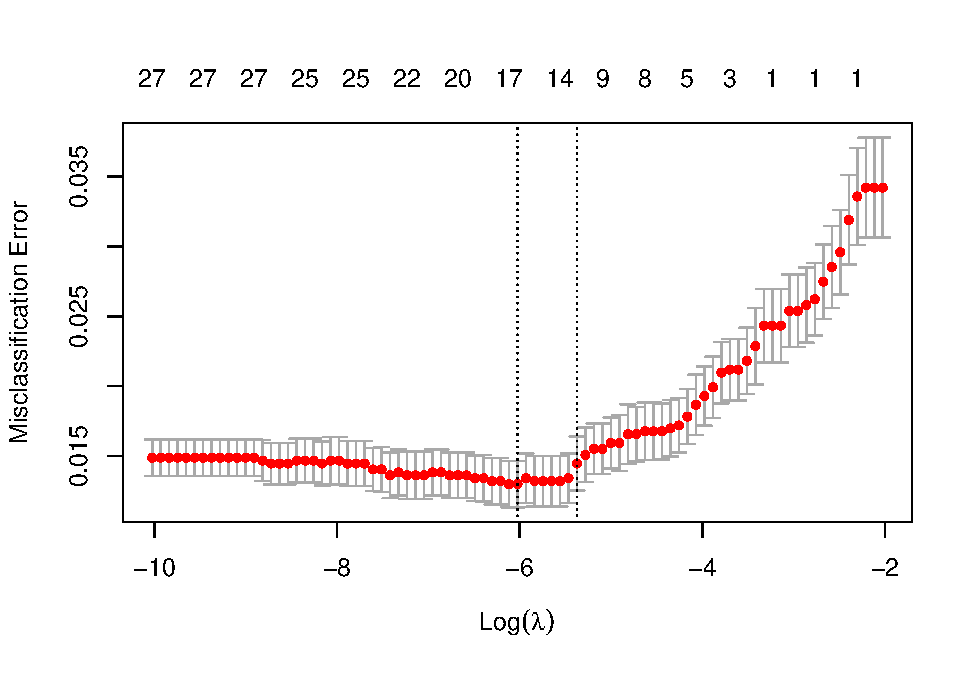
\includegraphics{report_files/figure-latex/unnamed-chunk-10-1.pdf}

\begin{verbatim}
## [1] 0.002419841
\end{verbatim}

\begin{longtable}[]{@{}lr@{}}
\caption{LASSO Model Coefficients}\tabularnewline
\toprule\noalign{}
Variable & Coefficient \\
\midrule\noalign{}
\endfirsthead
\toprule\noalign{}
Variable & Coefficient \\
\midrule\noalign{}
\endhead
\bottomrule\noalign{}
\endlastfoot
(Intercept) & -7.516 \\
num\_all\_star & 0.554 \\
num\_season & 0.000 \\
dpoy & 0.108 \\
mip & -0.080 \\
nba.roy & 0.000 \\
smoy & 0.590 \\
All.Defense.1st & 0.362 \\
All.Defense.2nd & -0.109 \\
All.NBA.1st & 0.123 \\
All.NBA.2nd & 0.434 \\
All.NBA.3rd & 0.000 \\
All.Rookie.1st & 0.010 \\
All.Rookie.2nd & 0.000 \\
trb & 0.000 \\
ast & 0.000 \\
stl & 0.000 \\
g & 0.016 \\
gs & -0.007 \\
ft\_percent & 0.000 \\
trb\_per\_game & 0.033 \\
ast\_per\_game & 0.240 \\
stl\_per\_game & 0.000 \\
blk\_per\_game & 0.000 \\
tov\_per\_game & -0.628 \\
pf\_per\_game & 0.626 \\
pts\_per\_game & 0.081 \\
mvp\_flag1 & 1.281 \\
\end{longtable}

\begin{longtable}[]{@{}lr@{}}
\caption{Ridge Model Coefficients}\tabularnewline
\toprule\noalign{}
Variable & Coefficient \\
\midrule\noalign{}
\endfirsthead
\toprule\noalign{}
Variable & Coefficient \\
\midrule\noalign{}
\endhead
\bottomrule\noalign{}
\endlastfoot
(Intercept) & -7.187 \\
num\_all\_star & 0.348 \\
num\_season & 0.030 \\
dpoy & 0.205 \\
mip & -0.858 \\
nba.roy & -0.059 \\
smoy & 0.598 \\
All.Defense.1st & 0.386 \\
All.Defense.2nd & -0.186 \\
All.NBA.1st & 0.294 \\
All.NBA.2nd & 0.571 \\
All.NBA.3rd & 0.231 \\
All.Rookie.1st & 0.360 \\
All.Rookie.2nd & 0.293 \\
trb & 0.000 \\
ast & 0.000 \\
stl & 0.000 \\
g & 0.012 \\
gs & -0.013 \\
ft\_percent & 0.412 \\
trb\_per\_game & 0.087 \\
ast\_per\_game & 0.211 \\
stl\_per\_game & -0.310 \\
blk\_per\_game & -0.067 \\
tov\_per\_game & -0.387 \\
pf\_per\_game & 0.350 \\
pts\_per\_game & 0.074 \\
mvp\_flag1 & 1.325 \\
\end{longtable}

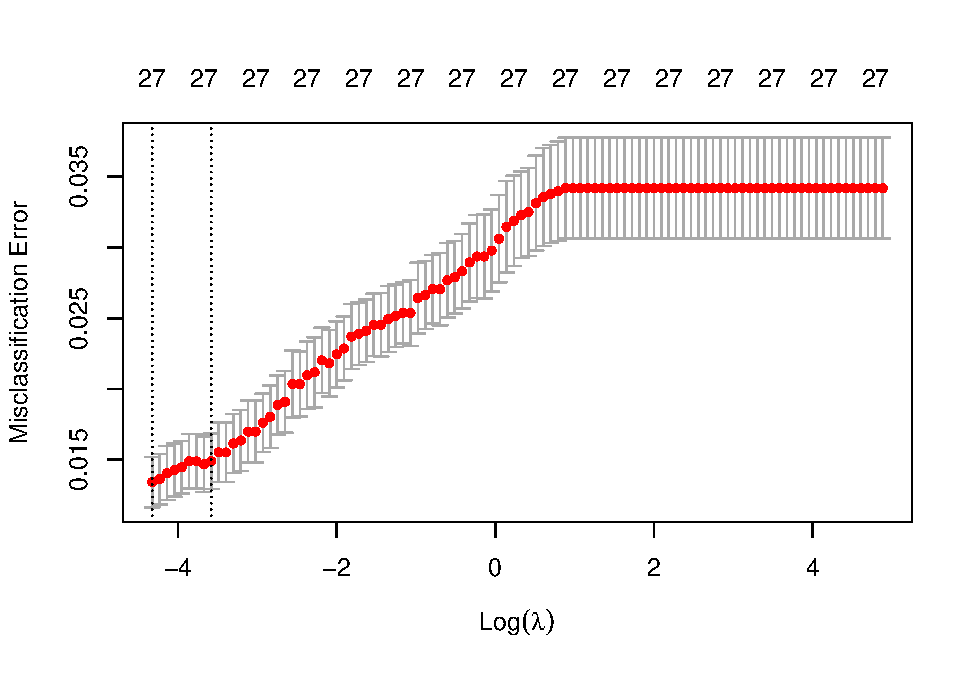
\includegraphics{report_files/figure-latex/unnamed-chunk-15-1.pdf}

\begin{verbatim}
## [1] 0.01321784
\end{verbatim}

\begin{Shaded}
\begin{Highlighting}[]
\NormalTok{cv\_lasso}\SpecialCharTok{$}\NormalTok{cvm[cv\_lasso}\SpecialCharTok{$}\NormalTok{lambda }\SpecialCharTok{==}\NormalTok{ cv\_lasso}\SpecialCharTok{$}\NormalTok{lambda.min]}
\end{Highlighting}
\end{Shaded}

\begin{verbatim}
## [1] 0.01300336
\end{verbatim}

\begin{Shaded}
\begin{Highlighting}[]
\NormalTok{cv\_ridge}\SpecialCharTok{$}\NormalTok{cvm[cv\_ridge}\SpecialCharTok{$}\NormalTok{lambda }\SpecialCharTok{==}\NormalTok{ cv\_ridge}\SpecialCharTok{$}\NormalTok{lambda.min]}
\end{Highlighting}
\end{Shaded}

\begin{verbatim}
## [1] 0.01342282
\end{verbatim}

\section{Results}\label{results}

\begin{Shaded}
\begin{Highlighting}[]
\NormalTok{x\_test }\OtherTok{\textless{}{-}} \FunctionTok{model.matrix}\NormalTok{(}\SpecialCharTok{\textasciitilde{}}\NormalTok{ ., }\AttributeTok{data =}\NormalTok{ test\_model)[, }\SpecialCharTok{{-}}\DecValTok{1}\NormalTok{]}
\end{Highlighting}
\end{Shaded}

\begin{Shaded}
\begin{Highlighting}[]
\NormalTok{pred }\OtherTok{\textless{}{-}} \FunctionTok{predict}\NormalTok{(cv\_lasso, }\AttributeTok{newx =}\NormalTok{ x\_test, }\AttributeTok{s =} \StringTok{"lambda.min"}\NormalTok{, }\AttributeTok{type =} \StringTok{"response"}\NormalTok{)}

\NormalTok{test\_with\_preds }\OtherTok{\textless{}{-}}\NormalTok{ test }\SpecialCharTok{\%\textgreater{}\%}
  \FunctionTok{mutate}\NormalTok{(}
    \AttributeTok{hof\_prob =} \FunctionTok{as.vector}\NormalTok{(pred)}
\NormalTok{  )}

\NormalTok{test\_with\_preds }\OtherTok{\textless{}{-}}\NormalTok{ test\_with\_preds }\SpecialCharTok{\%\textgreater{}\%}
  \FunctionTok{select}\NormalTok{(player, hof\_prob) }\SpecialCharTok{\%\textgreater{}\%}
  \FunctionTok{distinct}\NormalTok{(player, }\AttributeTok{.keep\_all =} \ConstantTok{TRUE}\NormalTok{) }\SpecialCharTok{\%\textgreater{}\%} 
  \FunctionTok{arrange}\NormalTok{(}\FunctionTok{desc}\NormalTok{(hof\_prob))}
\end{Highlighting}
\end{Shaded}

\begin{Shaded}
\begin{Highlighting}[]
\NormalTok{test\_with\_preds}
\end{Highlighting}
\end{Shaded}

\begin{verbatim}
## # A tibble: 563 x 2
##    player                hof_prob
##    <chr>                    <dbl>
##  1 LeBron James             1.00 
##  2 Chris Paul               1.00 
##  3 Kevin Durant             1.00 
##  4 Giannis Antetokounmpo    0.995
##  5 Stephen Curry            0.995
##  6 Russell Westbrook        0.992
##  7 James Harden             0.989
##  8 Anthony Davis            0.949
##  9 Nikola Jokić             0.948
## 10 Damian Lillard           0.935
## # i 553 more rows
\end{verbatim}

\section{Discussion}\label{discussion}

No Rudy Gobert

\subsection{Limitations}\label{limitations}

\subsection{Next Steps}\label{next-steps}

\section{Appendix}\label{appendix}

\url{https://www.sportingnews.com/us/nba/news/michael-jordan-vs-lebron-james-goat-debate/sl8xdozy5u1m1s4t5m3npeqo1}

\url{https://www.kaggle.com/datasets/sumitrodatta/nba-aba-baa-stats?select=Player+Career+Info.csv}

\end{document}
